\section{Polsby-Popper}\label{sec:pp}

The first compactness score we analyze is the \textit{Polsby-Popper score}, which takes the form of an \textit{isoperimetric quotient}, meaning it measures how much area a region's perimeter encloses, relative to all other regions with the same perimeter.
\mute{
\begin{definition}\label{def:pp}
The Polsby-Popper score of a region $\Omega$ is defined to be $$\mathrm{PP}(\Omega) = \frac{4\pi \cdot\mathrm{area}(\Omega)}{\mathrm{perim}(\Omega)^2}$$ and takes the form of an \textit{isoperimetric quotient} \abn{what's an isoperimetric quotient?}.  
\end{definition}
It's easy to check that among all regions in the plane with a fixed area, a circle of that area has the shortest perimeter, and equivalently, the Polsby-Popper score for a circle is 1.  We can analogously define the score on the sphere by transferring this intuition of isoperimetry.  In this first attempt, we transfer this notion directly to the sphere, and define the Polsby-Popper score on the sphere to be exactly the function in Definition~\ref{def:pp}. }
\abn{Rewrote Polsby-Popper intro to be more formulas and less words}\zs{looks good. leaving the comment here so we know something changed.}
\begin{definition}\label{def:pp}
The Polsby-Popper score of a region $\Omega$ is defined to be $$\mathrm{PP}_X(\Omega) = \frac{4\pi \cdot\mathrm{area}_X(\Omega)}{\mathrm{perim}_X(\Omega)^2}$$
Where $X$ is either the sphere $S$ or the plane $\R^2$, and $\mathrm{area}_X$ and 
$\mathrm{perim}_X$ are the area and perimeter 
respectively of $A$ in $X$.
\end{definition}
\begin{remark}
It is a classical theorem that for any 
reigon $A$ for which $\mathrm{PP}_{\R^2}(A)$ is defined,
$$
\mathrm{PP}_{\R^2}(A)\le 1
$$

with equality if and only if $A$ is a circle. In particular, the Polsby-Popper score is scale-invariant in the plane.  Both of these observations follow from the \textit{isoperimetric inequality} in the plane, which we state i the following lemma.
\begin{lemma}
If $\Omega$ is a region in the plane, then $4\pi\cdot\mathrm{area}(\Omega)\leq \mathrm{perim}(\Omega)^2$, with equality if and only if $\Omega$ is a circle.
\end{lemma}
\end{remark}
\mute{
It's easy to check that among all regions in the plane with a fixed area, a circle of that area has the shortest perimeter, and equivalently, the Polsby-Popper score for a circle is 1.  We can analogously define the score on the sphere by transferring this intuition of isoperimetry.  In this first attempt, we transfer this notion directly to the sphere, and define the Polsby-Popper score on the sphere to be exactly the function in Definition~\ref{def:pp}.

One concerning aspect of using this function on the sphere is that it is not a proper compactness measure.  If we consider a region on the sphere which is the whole sphere minus a small cap, the Polsby-Popper score is very, very large, and it grows without bound as we shrink the deleted portion, whereas the Polsby-Popper score of the image of any region under any projection is at most one.  Continuing down this lane of reasoning, since a projection needs to preserve maximizers of the score ordering, and there is no maximizer of the Polsby-Popper score on the sphere, we know immediately that if an order-preserving map projection $\varphi$ exists, that there can't be a region $\Omega$ on the sphere such that $\varphi(\Omega)$ is a circle in the plane.
But this is a contradiction, since we can just take a circle $C$ in the plane and look at $\varphi^{-1}(C)$, which must be some region on the sphere.

To avoid this, what if we restrict our attention to regions contained in the half-sphere?  As it turns out, this doesn't really resolve the problem.  To begin, we begin by stating the \textit{isoperimetric inequality on the sphere}.\footnote{For a more detailed treatment of isoperimetry, see \cite{osserman1979bonnesen} and \cite{rado}.}
}
\mute{It turns out that a similar fact can be 
stated for the sphere \cite{osserman1979bonnesen}, \cite{rado}:}
An isoperimetric inequality for the sphere exists, and we state it as the following lemma.  For a more detailed treatment of isoperimetry in general, see \cite{osserman1979bonnesen}, and for a proof of this inequality for the sphere, see \cite{rado}.
\zs{rewrote slightly}
\begin{lemma}
	If $\Omega$ is a region on the \mute{half-sphere} sphere with area $A$ and perimeter $P$, then $P^2\geq A^2-4\pi A$ with equality if and only if $\Omega$ is a spherical cap.
\end{lemma}
A consequence of this is that among all regions on the sphere with a fixed area $A$, a spherical cap with area $A$ has the shortest perimeter.  
%\lsn{ It feels weird to  me to call this theorem a "lemma"}
%\zs{I stated it as a lemma because I don't think we need to or even should be proving isoperimetric inequalities in here.  We can talk a little more about the audience, but it's one of those things that's intuitively true, but in order to get a rigorous proof, you need a few pages of symbol chasing and worrying about edge cases.  Maybe we can put a proof in an appendix if we feel like we need to include it?}

We need one more lemma, which we prove by computation, which demonstrates that the Polsby-Popper score is not scale-invariant on the sphere.
\abn{made ppscale lemma more concise} \zs{\checkmark}
\mute{
\begin{lemma}\label{lem:ppscale}
Let $A$ and $B$ be two caps on the half-sphere with $\mathrm{area}(A)\gneq \mathrm{area}(B)$.  Then the Polsby Popper score of $A$ is greater than that of $B$.
\end{lemma}

\begin{figure}
\centering
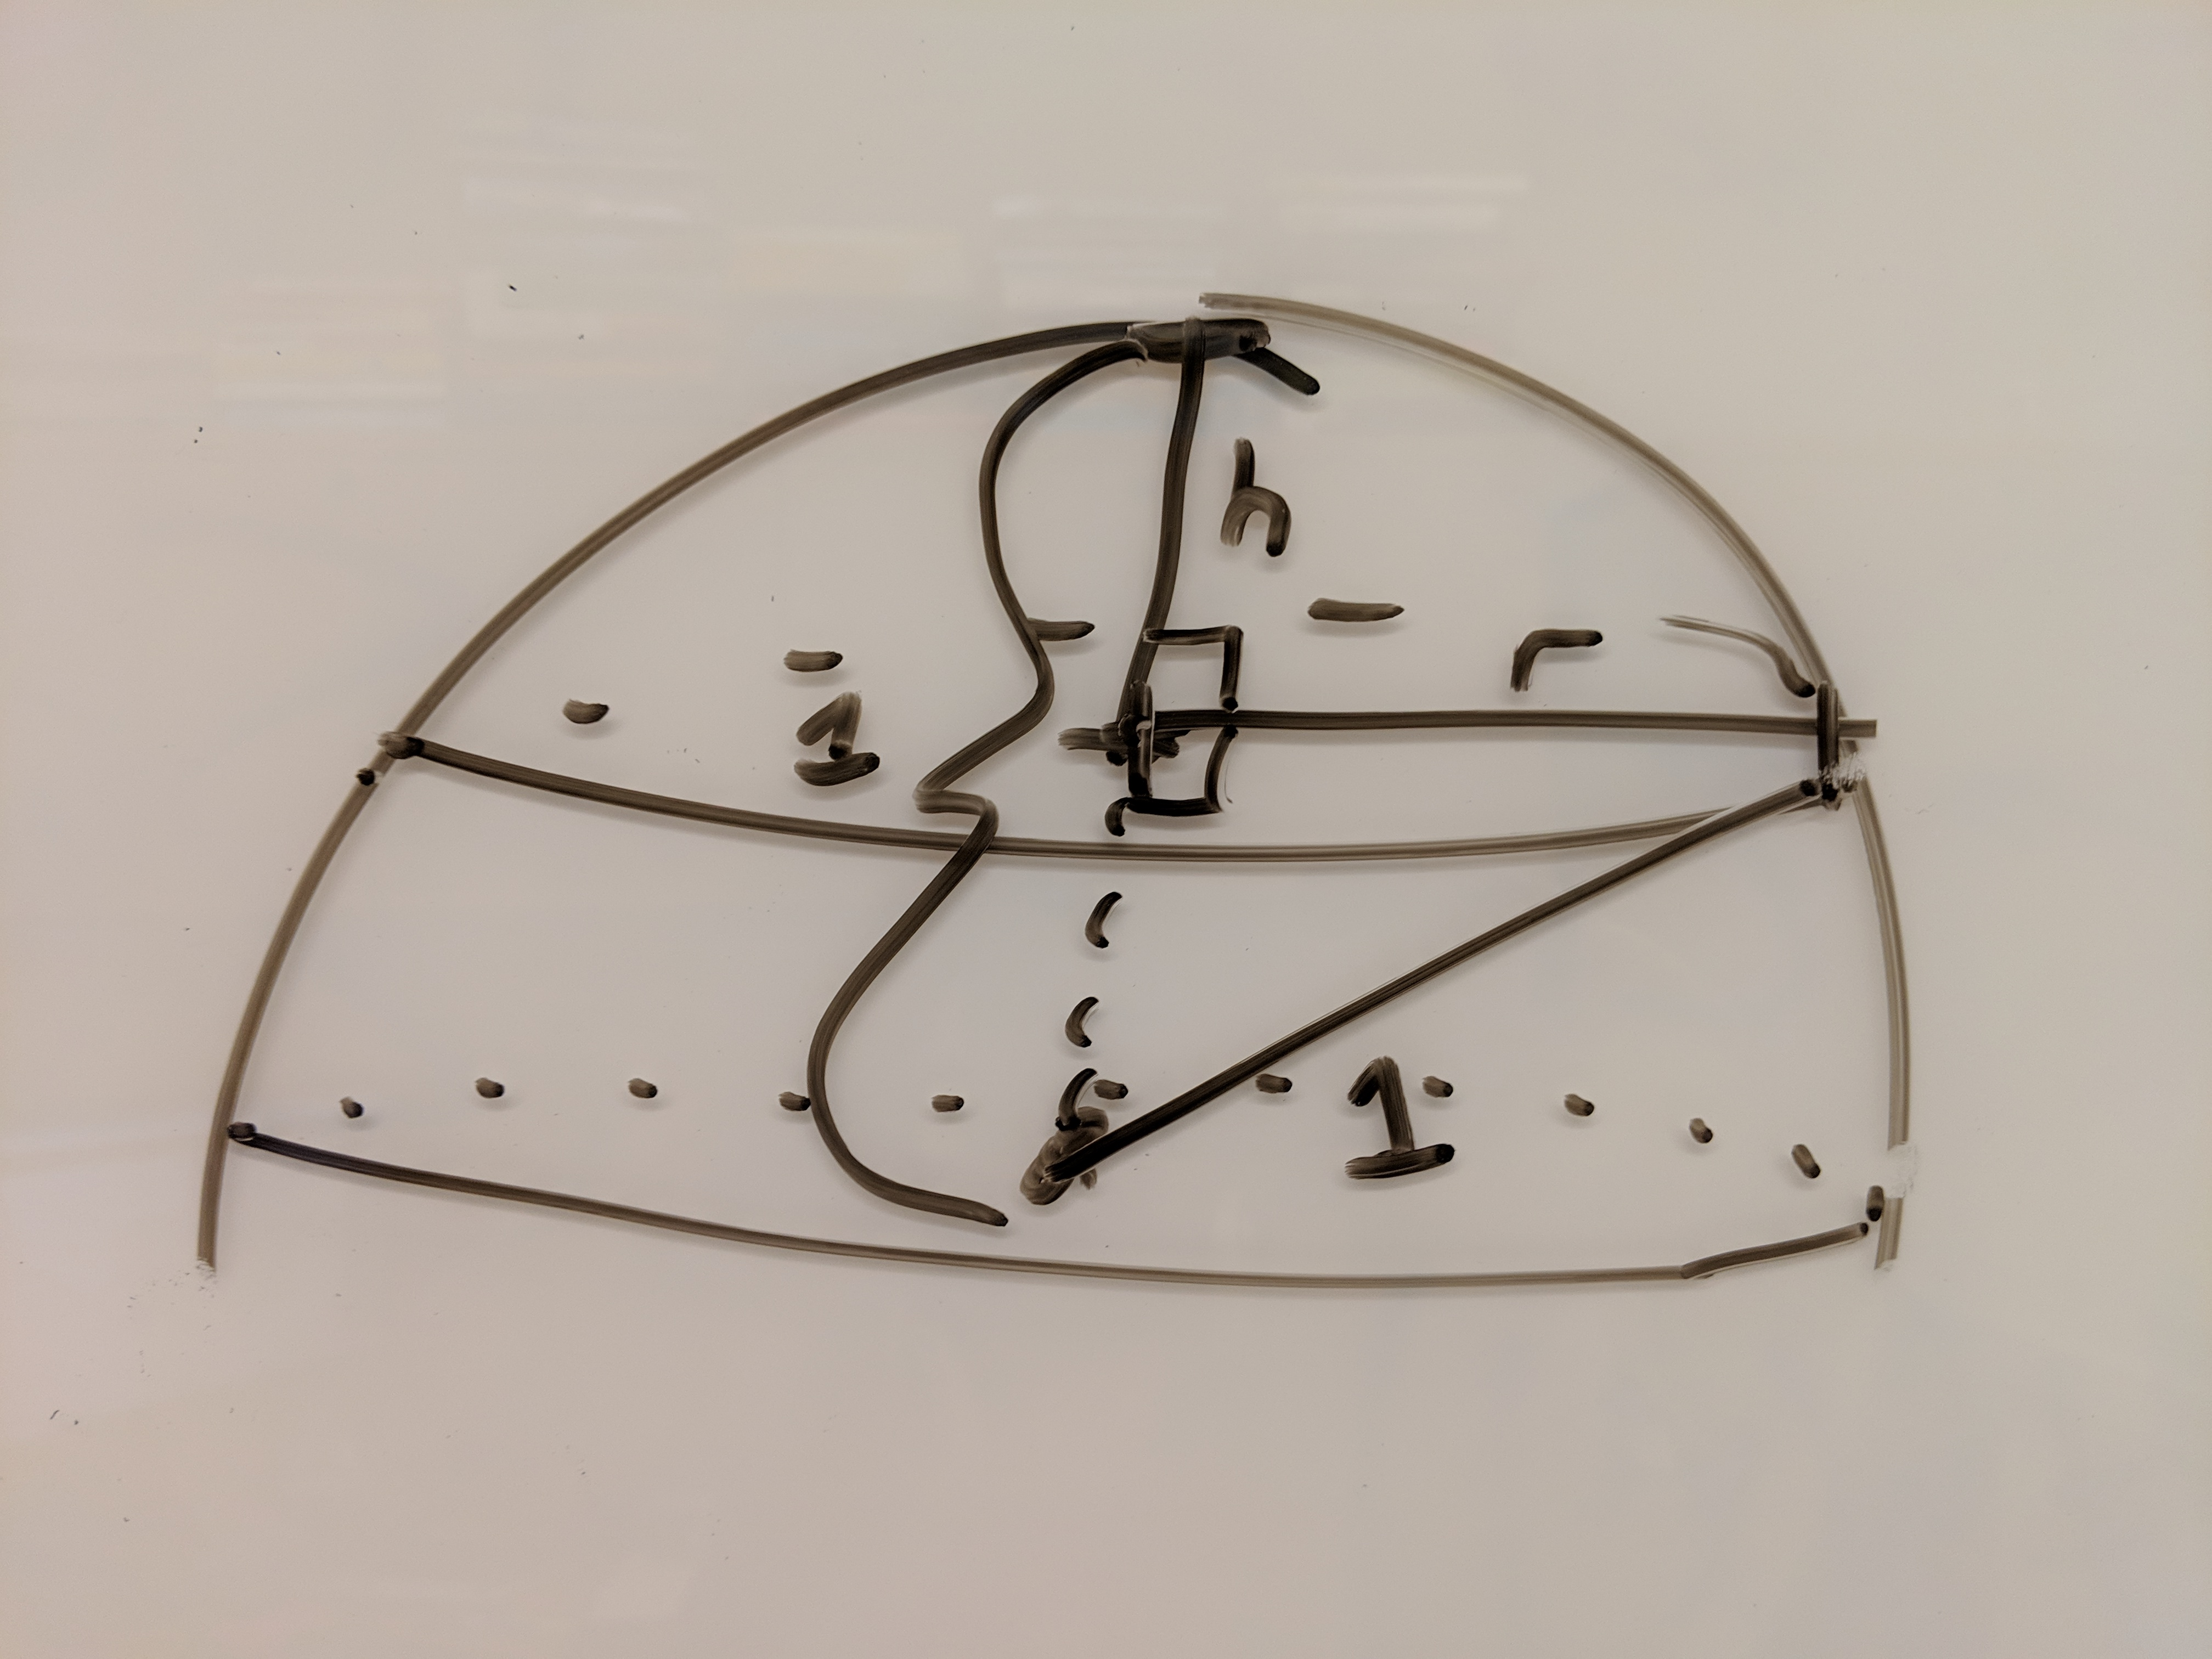
\includegraphics[width=.5\textwidth]{figs/spherical_cap.jpg}\\[1.5em]
\caption{ The height and radius of a spherical cap. }
\label{fig:caphr}
\end{figure}

\begin{proof}
Let $h_A$ and $h_B$ denote the heights of the caps $A$ and $B$, respectively, and $r_A$ and $r_B$ the radii (see Figure~\ref{fig:caphr}).  Since $\mathrm{area}(A)> \mathrm{area}(B)$, we know that $h_A>h_B$ and $r_A>r_B$.  

Since the radius of the sphere is known, we can write the $r$'s in terms of the $h$'s as 

$$r^2= 2h-h^2$$

Then, using well-known formulas, we know 

$$\mathrm{perim}(A) = 2\pi r_A = 2\pi \sqrt{2h_A-h_A^2}$$
$$\mathrm{perim}(B) = 2\pi r_B = 2\pi \sqrt{2h_B-h_B^2}$$

and

$$\mathrm{area}(A) = \pi(r_A^2+h_A^2) = \pi(2h_A-h_A^2 +h_A^2) = \pi(2h_A)$$
$$\mathrm{area}(B) = \pi(r_B^2+h_B^2) = \pi(2h_B-h_A^2 +h_B^2) = \pi(2h_B)$$

We can plug these expressions into the formula for the Polsby-Popper score to get

$$\mathrm{PP}(A) = \frac{4\pi (2\pi h_A) }{4 \pi^2 (2h_A-h_A^2)} = \frac{2}{2-h_A}$$
$$\mathrm{PP}(B) = \frac{4\pi (2\pi h_B) }{4 \pi^2 (2h_B-h_B^2)} = \frac{2}{2-h_B}$$

Since $h_A>h_B$, $\mathrm{PP}(A)$ must be greater than $\mathrm{PP}(B)$, which is what we wanted to prove,

\end{proof}
}
\begin{lemma}\label{lem:ppscale}
Let $S$ be the unit sphere, and let $\kappa(h)$ be the cap at height $h$ (i.e. the region comprised of all points whose $z$-coordinate is greater than $1-h$, where we imagine the sphere as being embedded in $\R^3$, centered at the origin) Then $\mathrm{PP}(\kappa(h))$ is a monotonically increasing function of $h$.
\end{lemma}
\zs{$A$ was a little overloaded, so I changed it to $\kappa$ \smiley{}}
\begin{figure}
\centering
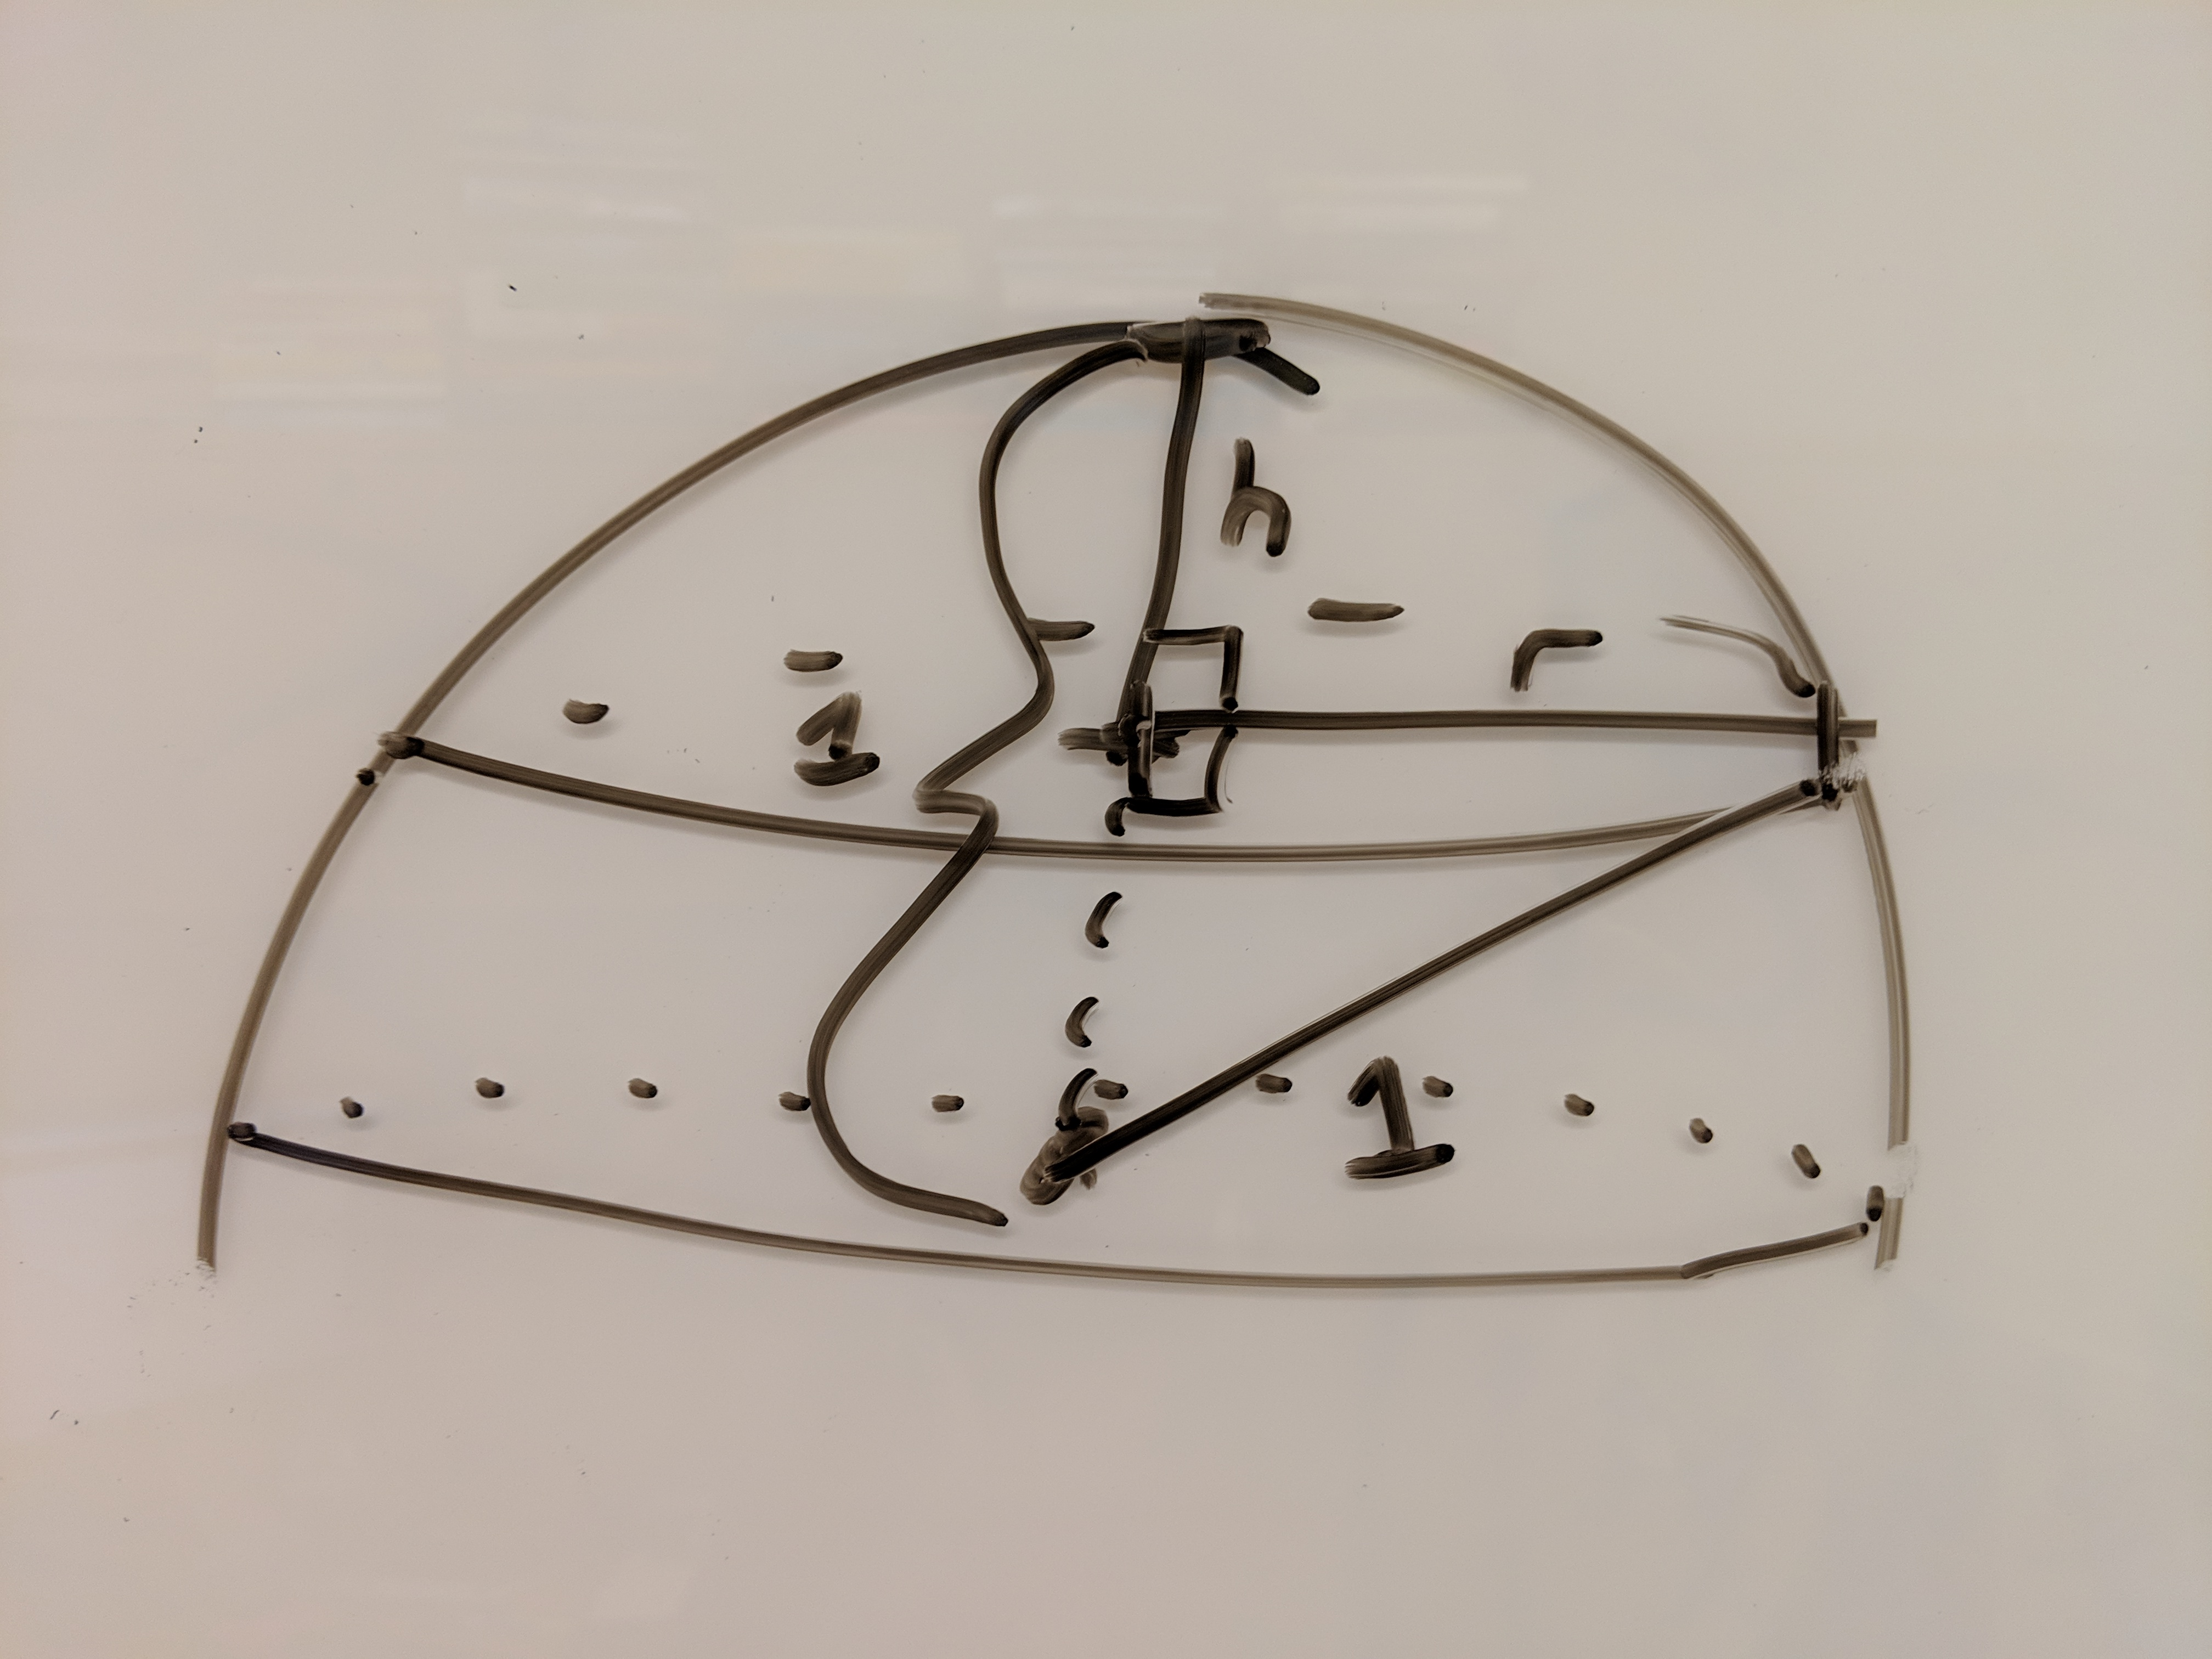
\includegraphics[width=.5\textwidth]{figs/spherical_cap.jpg}\\[1.5em]
\caption{ The height and radius of a spherical cap. }
\label{fig:caphr}
\end{figure}

\begin{proof}
Let $r(h)$ be the radius of the circle bounding $\kappa(h)$, and since we are working on the unit sphere, we know the radius of that sphere is equal to 1. We compute:
\begin{align*}
1 &= r(h)^2 + (1-h)^2 \text {, by right triangle trigonometry}\\ 
&= r(h)^2 + 1 - 2h+h^2
\end{align*}
Rearranging, we get that $r(h)^2= 2h-h^2$, which we can plug in to the standard formula for perimeter:
$$\mathrm{perim}_S(\kappa(h)) = 2\pi r(h) = 2\pi \sqrt{2h-h^2}$$

Computing the area of the spherical cap uses the fact that the cylindrical projection is area-preserving, and thus:
\zs{I think there's a better explanation than just asserting the existence of a projection that does this.  What about `Archimedes showed that the lateral surface area of a cylinder with radius $1$ and height $2$ is the same as the surface area of the spher, and that the lateral projection (do figure) from the sphere onto the cylinder preserves area.  Using this, we have that the area of a spherical cap at height $h$ is'}
$$
\mathrm{area}_S(\kappa(h)) = 2\pi h
$$
We can plug these expressions into the formula for the Polsby-Popper score to get
$$\mathrm{PP}_S(\kappa(h)) = \frac{4\pi (2\pi h) }{4 \pi^2 (2h-h^2)} = \frac{2}{2-h}$$
Which is a monotonically increasing function of $h$.
\end{proof}
\begin{corollary}\label{cor:capscale}
On the sphere, Polsby-Popper scores of caps are monotonically increasing with area
\end{corollary}
Using this, we can show the main theorem of this section, that no map projection from the half-sphere to the plane can preserve the ordering of Polsby-Popper scores for all regions.  

%\lsn{I think this is not the right statement / proof. See my email.}







\begin{theorem}\label{thm:dpp}
	If $\varphi$ is a map projection from the half-sphere to the plane, then there are two regions $A$ and $C$ in the half sphere such that the Polsby-Popper score of $C$ is greater than that of $A$ in the sphere, but the Polsby-Popper score of $\varphi(A)$ is greater than that of $\varphi(C)$ in the plane.
\end{theorem}
\begin{figure}\label{fig:dpp}
\centering
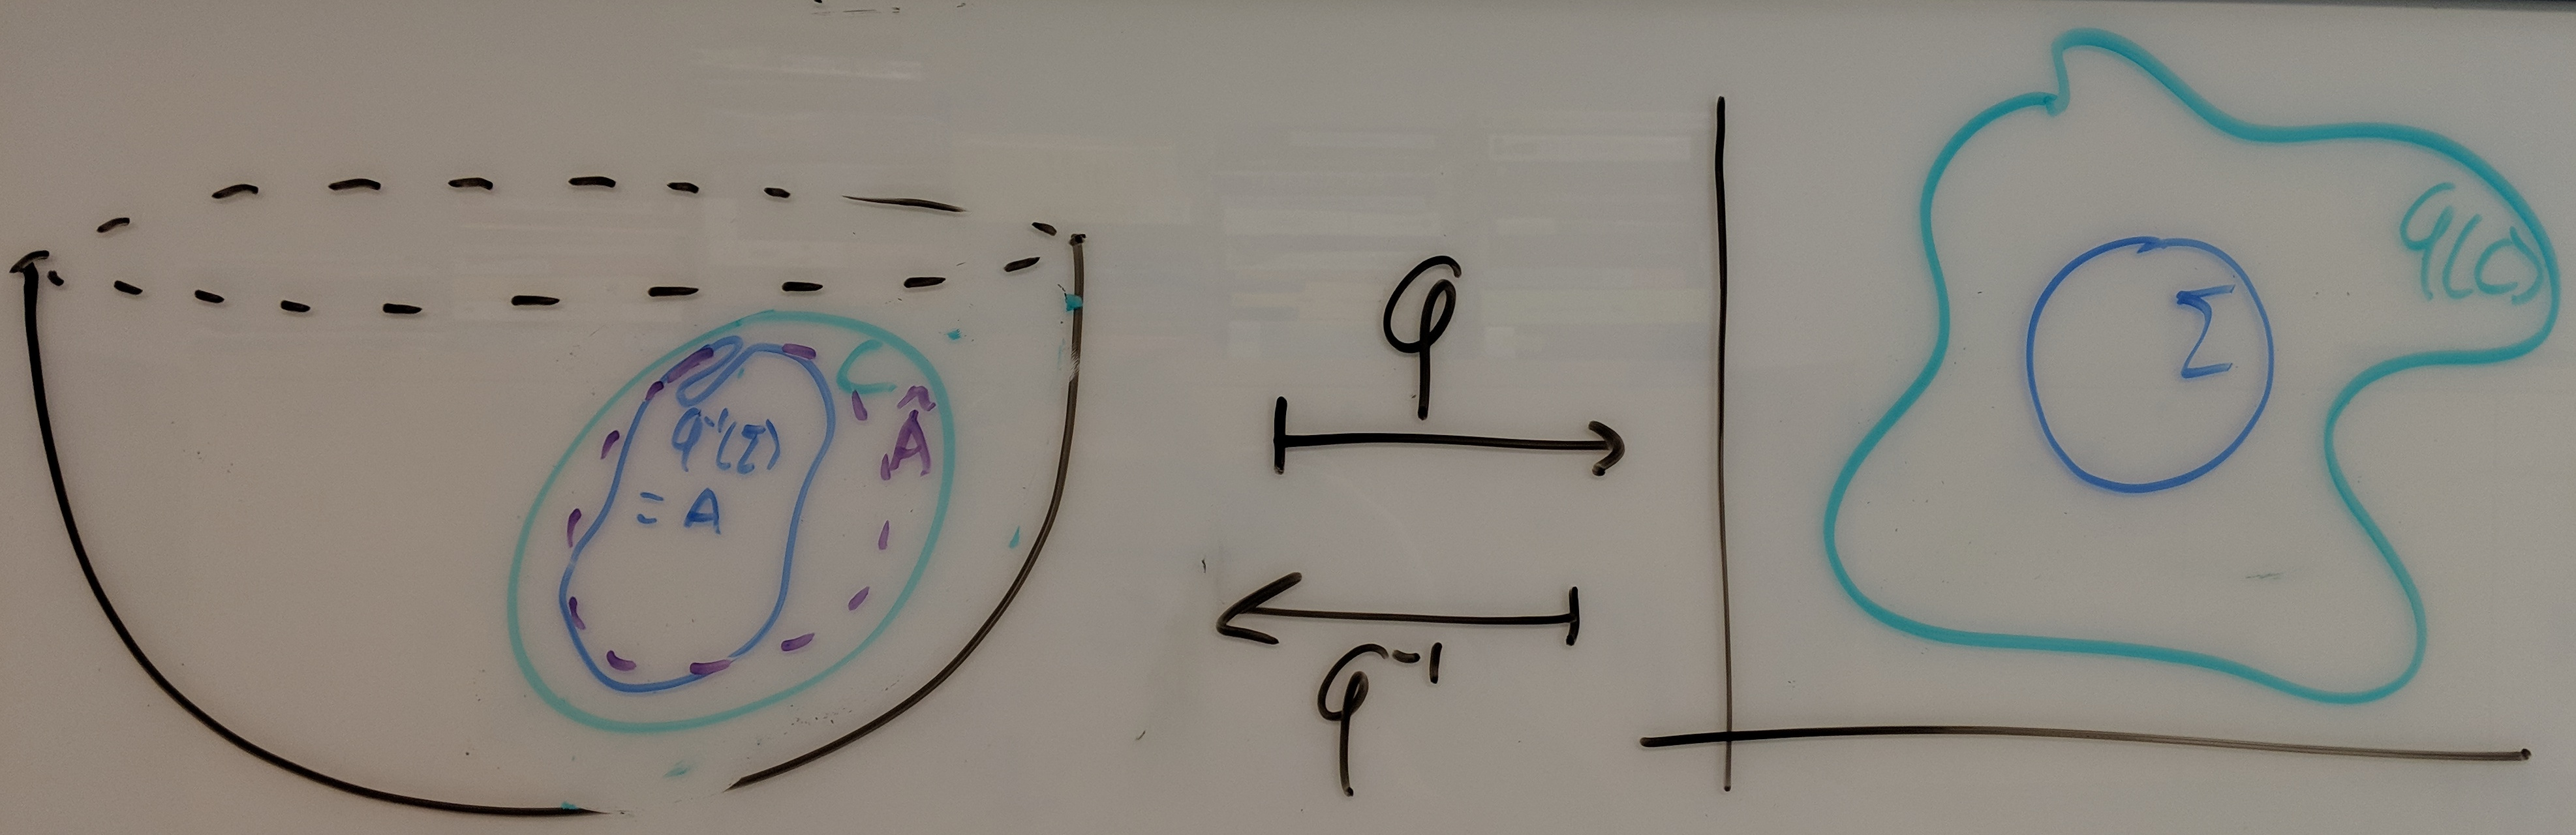
\includegraphics[width=.9\textwidth]{figs/dumb_pp_cropped.jpg}\\[1.5em]
\caption{ The construction of regions $A$, $C$, and $\hat{A}$ in the proof of Theorem~\ref{thm:dpp}.}
\end{figure}


\begin{proof}

	Let $\varphi$ be a map projection, and take $C$ to be a cap in the half-sphere. Let $\Sigma$ be a circle in the plane such that $\Sigma \subsetneq \varphi(C)$ and let $A=\varphi^{-1}(\Sigma)$ (see Figure~\ref{fig:dpp}).

	%\lsn{It doesn't depend on the preimage of $\Sigma$ not being a cap, because the preimage of $\Sigma$ has less area thatn $C$, so it's polsby popper score will be strictly worse.  I think this computation is necessary -- it's in the original doc. Also see my email.}

	The proof follows by inspection of the properties of these regions.
	
	Since $\Sigma$ is a circle, it maximizes the Polsby-Popper score in the plane, but $A$ does not do so in the sphere.  To see this, take $\hat{A}$ to be a cap in the sphere with area equal to that of $A$.  Since caps maximize the Polsby-Popper score in the sphere for a fixed area, we know that $\mathrm{PP}_S(\hat{A})\geq \mathrm{PP}_S(A)$.  Since map projections preserve containment, $\Sigma\subsetneq \varphi(C)$ implies that $A\subsetneq C$.  
	
	By construction, $\mathrm{area}(\hat{A})=\mathrm{area}(A)$ but $\mathrm{area}(A) \lneq \mathrm{area}(C)$, so $\mathrm{area}(\hat{A})< \mathrm{area}(C)$, which means that $\hat{A}$ is a cap with height and radius strictly smaller than that of $C$.
	
	By \abn{changed "by Lemma" to "by corollary to lemma"} \zs{changed ref} Corollary~\ref{cor:capscale}, we know that $\mathrm{PP_S}(\hat{A})< \mathrm{PP_S}(C)$, and combining this with the earlier inequality, we get
	
	$$\mathrm{PP_S}({A})\leq \mathrm{PP_S}(\hat{A})< \mathrm{PP_S}(C).$$
	
	Since $\Sigma = \varphi(A)$ maximizes the Polsby-Popper score in the plane, but $A$ does not do so in the sphere, we have shown that $\varphi$ does not preserve the maximal elements in the score ordering, and therefore it cannot preserve the ordering itself.
\end{proof}

The reason why every map projection fails to preserve the ordering of Polsby-Popper scores is because the score itself is constructed from the \textit{planar} notion of isoperimetry, and there is no reason to expect this formula to move nicely back and forth between the sphere and the plane.  This proof crucially exploits a scale invariance present in the plane but not the sphere.  If we consider any circle in the plane, it's Polsby-Popper score is definitionally equal to one, but that is not true of every cap in the sphere.  This naturally raises the question of whether being more careful, and defining a compactness score which uses the isoperimetric quotient of the surface the region is actually in will evade this problem.  We show later that it does resolve the issue of scale-noninvariance, but it is still induces an ordering which is not preserved by any map projection.  We address this in Section~\ref{sec:isoper}, as it uses on machinery we develop in the interceding sections.